\section{A grid network of PING oscillators}

The external stimulation of neural circuits, such as induction of electrical currents, produces electrical transmembrane currents resulting in neural membrane potential fluctuations \cite{IzhikevichBook2004:2}. Input currents surpassing a threshold give rise to action potential or a spike, an abrupt and transient change of membrane potential that propagates to other neurons. Postsynaptic neurons receiving stimulation from presynaptic neurons fire (i.e. generate spike(s)) if the summation of their presynaptic input again surpasses a threshold. Afterward, the neuron resets its membrane potential. The spiking state of the neuron can be transient or stable depending on the type of neuron or the strength of the input current (or pulse). In addition, the presynaptic input can be inhibitory or excitatory depending on the type of presynaptic neurons. Inhibitory neurons release neurotransmitters that inhibit, or restrict, the firing of an action potential; excitatory neurons release neurotransmitters that fire an action potential in the postsynaptic neuron.

In a pyramidal interneuron network gamma (PING) model, the interplay between a group of  excitatory (e.g. pyramidal cells) and inhibitory neurons (e.g. fast-spiking basket cells) give rise to synchronous rhythmic spikes in gamma frequency range (25-80 Hz)  \cite{Whittington2000}, \cite{Borgers2003}. The schematic architecture of the network is presented in Figure \ref{fig:single-ping}.

\begin{figure}[!htp]
    \centering
    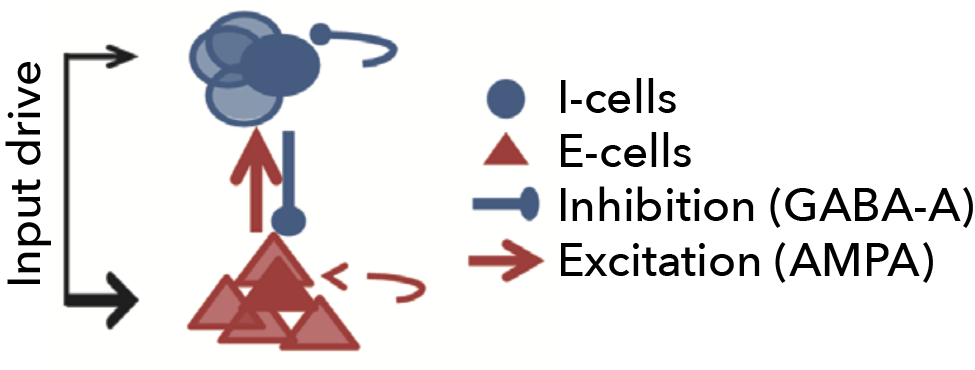
\includegraphics[width=0.5\textwidth]{assets/images/single-ping.png}
    \caption{Schematic architecture of the pyramidal-interneuron network gamma (PING) \cite{Lowet2015}.
    \todo{why the input drive arrow is much thicker to excitatory neurons?}}
    \label{fig:single-ping}
\end{figure}

Specifically, in this network, the gamma oscillations are instigated by the input to excitatory neurons followed by inhibitory feedback \cite{Whittington2000}. In conditions of sufficient excitatory drive, pyramidal cells excite fast-spiking (FS) neurons. FS neurons then become depolarized and inhibit the pyramidal neurons, thus creating a loop. The suppression of pyramidal cells stops the depolarization of FS cells and, therefore, stops their inhibitory effect (i.e. suppression of pyramidal cells). This provides a time interval for pyramidal cells to fire again until they cause their inhibition through FS cells again. Then the excitatory cells spike again, repeating the cycle \cite{Kopell2011}.

\subsection{The network}
\label{sec:grid-network}

The network considered in this thesis is an oscillatory network that represents a patch of neural networks in V1. Each PING network stands for an oscillator reflecting a neural circuit in V1, which interacts with other neural circuits in this area through lateral connections.
In this oscillatory network, a group of oscillators is arranged in a $n \times n$ grid similar to the network illustrated in Figure \ref{fig:oscillatory-grid-graph}.

\begin{figure}[!htp]
    \centering
    \begin{tikzpicture}[
    arr/.style = { -{Stealth[ ]} },
    cnodeex/.style = {circle,thick,fill=main-color},
    cnodein/.style = {circle,thick,fill=sec-color},
    cframerounded/.style = {rounded corners=0.8cm, very thick, third-color},
]
        
    % vertices 1
    \begin{scope}
        \draw[cframerounded] (0.5, 0.7) rectangle (3.5, 2.5) {};
        
        \node[style=cnodeex] (Vex0) at (1, 2) {};
        \node[style=cnodeex] (Vex1) at (2, 2) {};
        \node[style=cnodeex] (Vex2) at (3, 2) {};
        
        \node[style=cnodein] (Vin3) at (1.5, 1) {};
        \node[style=cnodein] (Vin4) at (2.5, 1) {};
    \end{scope}
    
    % vertices 2
    \begin{scope}
        \draw[cframerounded] (4.5, 0.7) rectangle (7.5, 2.5) {};
        
        \node[style=cnodeex] (Vex5) at (5, 2) {};
        \node[style=cnodeex] (Vex6) at (6, 2) {};
        \node[style=cnodeex] (Vex7) at (7, 2) {};
        
        \node[style=cnodein] (Vin8) at (5.5, 1) {};
        \node[style=cnodein] (Vin9) at (6.5, 1) {};
    \end{scope}
    
    % vertices 3
    \begin{scope}
        \draw[cframerounded] (8.5, 0.7) rectangle (11.5, 2.5) {};
        
        \node[style=cnodeex] (Vex10) at (9, 2) {};
        \node[style=cnodeex] (Vex11) at (10, 2) {};
        \node[style=cnodeex] (Vex12) at (11, 2) {};
        
        \node[style=cnodein] (Vin13) at (9.5, 1) {};
        \node[style=cnodein] (Vin14) at (10.5, 1) {};
    \end{scope}
    
    % vertices 4
    \begin{scope}
        \draw[cframerounded] (0.5, 3.7) rectangle (3.5, 5.5) {};
        
        \node[style=cnodeex] (Vex15) at (1, 5) {};
        \node[style=cnodeex] (Vex16) at (2, 5) {};
        \node[style=cnodeex] (Vex17) at (3, 5) {};
        
        \node[style=cnodein] (Vin18) at (1.5, 4) {};
        \node[style=cnodein] (Vin19) at (2.5, 4) {};
    \end{scope}
    
    % vertices 5
    \begin{scope}
        \draw[cframerounded] (4.5, 3.7) rectangle (7.5, 5.5) {};
        
        \node[style=cnodeex] (Vex20) at (5, 5) {};
        \node[style=cnodeex] (Vex21) at (6, 5) {};
        \node[style=cnodeex] (Vex22) at (7, 5) {};
        
        \node[style=cnodein] (Vin23) at (5.5, 4) {};
        \node[style=cnodein] (Vin24) at (6.5, 4) {};
    \end{scope}
    
    % vertices 6
    \begin{scope}
        \draw[cframerounded] (8.5, 3.7) rectangle (11.5, 5.5) {};
        
        \node[style=cnodeex] (Vex25) at (9, 5) {};
        \node[style=cnodeex] (Vex26) at (10, 5) {};
        \node[style=cnodeex] (Vex27) at (11, 5) {};
        
        \node[style=cnodein] (Vin28) at (9.5, 4) {};
        \node[style=cnodein] (Vin29) at (10.5, 4) {};
    \end{scope}
    
    % vertices 7
    \begin{scope}
        \draw[cframerounded] (0.5, 6.7) rectangle (3.5, 8.5) {};
        
        \node[style=cnodeex] (Vex30) at (1, 8) {};
        \node[style=cnodeex] (Vex31) at (2, 8) {};
        \node[style=cnodeex] (Vex32) at (3, 8) {};
        
        \node[style=cnodein] (Vin33) at (1.5, 7) {};
        \node[style=cnodein] (Vin34) at (2.5, 7) {};
    \end{scope}
    
    % vertices 8
    \begin{scope}
        \draw[cframerounded] (4.5, 6.7) rectangle (7.5, 8.5) {};
        
        \node[style=cnodeex] (Vex35) at (5, 8) {};
        \node[style=cnodeex] (Vex36) at (6, 8) {};
        \node[style=cnodeex] (Vex37) at (7, 8) {};
        
        \node[style=cnodein] (Vin38) at (5.5, 7) {};
        \node[style=cnodein] (Vin39) at (6.5, 7) {};
    \end{scope}
    
    % vertices 9
    \begin{scope}
        \draw[cframerounded] (8.5, 6.7) rectangle (11.5, 8.5) {};
        
        \node[style=cnodeex] (Vex40) at (9, 8) {};
        \node[style=cnodeex] (Vex41) at (10, 8) {};
        \node[style=cnodeex] (Vex42) at (11, 8) {};
        
        \node[style=cnodein] (Vin43) at (9.5, 7) {};
        \node[style=cnodein] (Vin44) at (10.5, 7) {};
    \end{scope}
    
    % =======================================================
    
    \begin{scope}[>={Stealth[black]}]
        % vertical 
        
        % 1 to 4
        \draw[->] (2.1, 2.5) to[bend right] (2.1, 3.7);
        \draw[->] (1.9, 3.7) to[bend right] (1.9, 2.5);
        
        % 4 to 7
        \draw[->] (2.1, 5.5) to[bend right] (2.1, 6.7);
        \draw[->] (1.9, 6.7) to[bend right] (1.9, 5.5);
        
        % 2 to 5
        \draw[->] (6.1, 2.5) to[bend right] (6.1, 3.7);
        \draw[->] (5.9, 3.7) to[bend right] (5.9, 2.5);
        
        % 5 to 8
        \draw[->] (6.1, 5.5) to[bend right] (6.1, 6.7);
        \draw[->] (5.9, 6.7) to[bend right] (5.9, 5.5);
        
        % 3 to 6
        \draw[->] (10.1, 2.5) to[bend right] (10.1, 3.7);
        \draw[->] (9.9, 3.7) to[bend right] (9.9, 2.5);
        
        % 6 to 9
        \draw[->] (10.1, 5.5) to[bend right] (10.1, 6.7);
        \draw[->] (9.9, 6.7) to[bend right] (9.9, 5.5);
        
        % horizontal
        
        % 1 to 2
        \draw[->] (3.5, 1.7) to[bend left] (4.5, 1.7);
        \draw[->] (4.5, 1.5) to[bend left] (3.5, 1.5);
        
        % 2 to 3
        \draw[->] (7.5, 1.7) to[bend left] (8.5, 1.7);
        \draw[->] (8.5, 1.5) to[bend left] (7.5, 1.5);
        
        % 4 to 5
        \draw[->] (3.5, 4.7) to[bend left] (4.5, 4.7);
        \draw[->] (4.5, 4.5) to[bend left] (3.5, 4.5);
        
        % 5 to 6
        \draw[->] (7.5, 4.7) to[bend left] (8.5, 4.7);
        \draw[->] (8.5, 4.5) to[bend left] (7.5, 4.5);
        
        % 7 to 8
        \draw[->] (3.5, 7.7) to[bend left] (4.5, 7.7);
        \draw[->] (4.5, 7.5) to[bend left] (3.5, 7.5);
        
        % 8 to 9
        \draw[->] (7.5, 7.7) to[bend left] (8.5, 7.7);
        \draw[->] (8.5, 7.5) to[bend left] (7.5, 7.5);
    \end{scope}
    
    % edges 
    \begin{scope}
        \path (Vex0) edge node {} (Vex1);
        \path (Vex0) edge[bend left=25] node {} (Vex2);
        \path (Vex0) edge node {} (Vin3);
        \path (Vex0) edge node {} (Vin4);
        \path (Vex1) edge node {} (Vex2);
        \path (Vex1) edge node {} (Vin3);
        \path (Vex1) edge node {} (Vin4);
        \path (Vex2) edge node {} (Vin3);
        \path (Vex2) edge node {} (Vin4);
        \path (Vin3) edge node {} (Vin4);
        \path (Vex5) edge node {} (Vex6);
        \path (Vex5) edge[bend left=25] node {} (Vex7);
        \path (Vex5) edge node {} (Vin8);
        \path (Vex5) edge node {} (Vin9);
        \path (Vex6) edge node {} (Vex7);
        \path (Vex6) edge node {} (Vin8);
        \path (Vex6) edge node {} (Vin9);
        \path (Vex7) edge node {} (Vin8);
        \path (Vex7) edge node {} (Vin9);
        \path (Vin8) edge node {} (Vin9);
        \path (Vex10) edge node {} (Vex11);
        \path (Vex10) edge[bend left=25] node {} (Vex12);
        \path (Vex10) edge node {} (Vin13);
        \path (Vex10) edge node {} (Vin14);
        \path (Vex11) edge node {} (Vex12);
        \path (Vex11) edge node {} (Vin13);
        \path (Vex11) edge node {} (Vin14);
        \path (Vex12) edge node {} (Vin13);
        \path (Vex12) edge node {} (Vin14);
        \path (Vin13) edge node {} (Vin14);
        \path (Vex15) edge node {} (Vex16);
        \path (Vex15) edge[bend left=25] node {} (Vex17);
        \path (Vex15) edge node {} (Vin18);
        \path (Vex15) edge node {} (Vin19);
        \path (Vex16) edge node {} (Vex17);
        \path (Vex16) edge node {} (Vin18);
        \path (Vex16) edge node {} (Vin19);
        \path (Vex17) edge node {} (Vin18);
        \path (Vex17) edge node {} (Vin19);
        \path (Vin18) edge node {} (Vin19);
        \path (Vex20) edge node {} (Vex21);
        \path (Vex20) edge[bend left=25] node {} (Vex22);
        \path (Vex20) edge node {} (Vin23);
        \path (Vex20) edge node {} (Vin24);
        \path (Vex21) edge node {} (Vex22);
        \path (Vex21) edge node {} (Vin23);
        \path (Vex21) edge node {} (Vin24);
        \path (Vex22) edge node {} (Vin23);
        \path (Vex22) edge node {} (Vin24);
        \path (Vin23) edge node {} (Vin24);
        \path (Vex25) edge node {} (Vex26);
        \path (Vex25) edge[bend left=25] node {} (Vex27);
        \path (Vex25) edge node {} (Vin28);
        \path (Vex25) edge node {} (Vin29);
        \path (Vex26) edge node {} (Vex27);
        \path (Vex26) edge node {} (Vin28);
        \path (Vex26) edge node {} (Vin29);
        \path (Vex27) edge node {} (Vin28);
        \path (Vex27) edge node {} (Vin29);
        \path (Vin28) edge node {} (Vin29);
        \path (Vex30) edge node {} (Vex31);
        \path (Vex30) edge[bend left=25] node {} (Vex32);
        \path (Vex30) edge node {} (Vin33);
        \path (Vex30) edge node {} (Vin34);
        \path (Vex31) edge node {} (Vex32);
        \path (Vex31) edge node {} (Vin33);
        \path (Vex31) edge node {} (Vin34);
        \path (Vex32) edge node {} (Vin33);
        \path (Vex32) edge node {} (Vin34);
        \path (Vin33) edge node {} (Vin34);
        \path (Vex35) edge node {} (Vex36);
        \path (Vex35) edge[bend left=25] node {} (Vex37);
        \path (Vex35) edge node {} (Vin38);
        \path (Vex35) edge node {} (Vin39);
        \path (Vex36) edge node {} (Vex37);
        \path (Vex36) edge node {} (Vin38);
        \path (Vex36) edge node {} (Vin39);
        \path (Vex37) edge node {} (Vin38);
        \path (Vex37) edge node {} (Vin39);
        \path (Vin38) edge node {} (Vin39);
        \path (Vex40) edge node {} (Vex41);
        \path (Vex40) edge[bend left=25] node {} (Vex42);
        \path (Vex40) edge node {} (Vin43);
        \path (Vex40) edge node {} (Vin44);
        \path (Vex41) edge node {} (Vex42);
        \path (Vex41) edge node {} (Vin43);
        \path (Vex41) edge node {} (Vin44);
        \path (Vex42) edge node {} (Vin43);
        \path (Vex42) edge node {} (Vin44);
        \path (Vin43) edge node {} (Vin44);
    \end{scope}
\end{tikzpicture}
    \caption{An example of a 3 $\times$ 3 oscillatory network arranged in a grid. The arrows represent pairwise connections between all neurons (only shown for neighbouring cells, exist for all neurons). All connections in the network represent a bidirectional interaction.}
    \label{fig:oscillatory-grid-graph}
\end{figure}

This oscillatory network can be represented as a complete weighted directed graph $D = (V, E)$, where the set of vertices $V$ represents all neurons in the network, and the set of edges $E$ represents the synapses. Structurally, the oscillatory network connects $n^2$ identical subgraphs, each representing a PING network. Each subgraph contains the same number of excitatory and inhibitory neurons. An example of such a subgraph is visualized in Figure \ref{fig:single-ping-graph}. 
The cost function $\cost: E \to \mathbb{R}$ for the graph $D$ that reflects the interactions between neurons is defined later in Equation (\ref{eq:cost-function}).

\begin{figure}[!htp]
    \centering
    \begin{tikzpicture}[
    arr/.style = { -{Stealth[ ]} },
    cnodeex/.style = {circle,thick,fill=main-color},
    cnodein/.style = {circle,thick,fill=sec-color},
    cframerounded/.style = {rounded corners=0.8cm, very thick, third-color},
]

    \begin{scope}
        \node (in) at (6, 6.6) {Excitatory neurons};
        \draw[cframerounded] (0, 4.3) rectangle (12, 6.3) {};
        \node[style=cnodeex] (Vex0) at (1, 5) {$v_0$};
        \node[style=cnodeex] (Vex1) at (6, 5) {$v_1$};
        \node[style=cnodeex] (Vex2) at (11, 5) {$v_2$};
        
        \node (in) at (6, 0) {Inhibitory neurons};
        \draw[cframerounded] (2.5, 0.5) rectangle (9.5, 2.1) {};
        \node[style=cnodein] (Vin3) at (3.5, 1.3) {$v_3$};
        \node[style=cnodein] (Vin4) at (8.5, 1.3) {$v_4$};
    \end{scope}
    
    \begin{scope}[>={Stealth[black]}]
        
        \path [->] (Vex0) edge[bend left=7] node {} (Vex1);
        \path [->] (Vex1) edge[bend left=7] node {} (Vex0);
        
        \path [->] (Vex0) edge[bend left=12] node {} (Vex2);
        \path [->] (Vex2) edge[bend right=18] node {} (Vex0);
        
        \path [->] (Vex1) edge[bend left=7] node {} (Vex2);
        \path [->] (Vex2) edge[bend left=7] node {} (Vex1);
        
        \path [->] (Vin3) edge[bend left=7] node {} (Vin4);
        \path [->] (Vin4) edge[bend left=7] node {} (Vin3);
        
        \path [->] (Vex0) edge[bend left=7] node {} (Vin3);
        \path [->] (Vin3) edge[bend left=7] node[below left] {$\cost_{(v_3 \to v_0)}$} (Vex0);
        
        \path [->] (Vex0) edge[bend left=7] node {} (Vin4);
        \path [->] (Vin4) edge[bend left=7] node {} (Vex0);
        
        \path [->] (Vex1) edge[bend left=7] node {} (Vin3);
        \path [->] (Vin3) edge[bend left=7] node {} (Vex1);
        
        \path [->] (Vex1) edge[bend left=7] node {} (Vin4);
        \path [->] (Vin4) edge[bend left=7] node {} (Vex1);
        
        \path [->] (Vex2) edge[bend left=7] node {} (Vin3);
        \path [->] (Vin3) edge[bend left=7] node {} (Vex2);
        
        \path [->] (Vex2) edge[bend left=7] node[below right] {$\cost_{(v_2 \to v_4)}$} (Vin4);
        \path [->] (Vin4) edge[bend left=7] node {} (Vex2);
    \end{scope}
\end{tikzpicture}
    \caption{An example of a PING network represented as graph with three excitatory and two inhibitory neurons. Each edge has a cost function but only two are displayed for aesthetic purposes.}
    \label{fig:single-ping-graph}
\end{figure}

\subsection{Neural dynamics}
\label{sec:neural-dynamics}

A common approach to systematically simulate a PING network involves the definition of neural dynamics through the Izhikevich type neuron model  \cite{Izhikevich2003}. Every neuron in a PING network is a dynamical system that can be described with a two-dimensional system of ordinary differential equations. 

The set of neurons can be separated in the following way: $V = \{ V_{\ex}, V_{\inh}\}$, where $V_{\ex}$ is a set of excitatory neurons, and $V_{\inh}$ - a set of inhibitory neurons, such that $V_{\ex} \cap V_{\inh} = \emptyset$.
Therefore, we can define $\type: V \to \{ \ex, \ \inh \}$ to be a function mapping a neuron to its type: $\ex$ corresponds to excitatory, and $\inh$ - to inhibitory neurons. Then, for all $v \in V$,
\begin{align}
    \frac{dp_v}{dt} =\ & 0.04 p_v^2 + 5p_v + 140 - r_v + I_v,
    \label{eq:Izhikevich-model-dv-dt} \\
    \frac{dr_v}{dt} =\ & \alpha_{\type(v)} \cdot (\beta_{\type(v)} p_v - r_v), \label{eq:Izhikevich-model-dr-dt} \\
    \text{if } p_v \geq\ & 30 \text{ mV, then } 
    \begin{cases}
        p_v \leftarrow \gamma_{\type(v)} \\
        r_v \leftarrow r_v + \zeta_{\type(v)}
    \end{cases}, 
    \label{eq:Izhikevich-model-p30}
\end{align}
where
\begin{itemize}
    \item $p$ represents the membrane potential of the neuron; 
    
    \item $r$ represents a membrane recovery variable; provides negative feedback to $p$;
    
    \item $\alpha$ describes the timescale of $r$;
    
    \item $\beta$ describes the sensitivity of $r$ to the subthreshold fluctuations of $p$;
    
    \item $\gamma$ describes the after-spike reset value of $p$;
    
    \item $\zeta$ describes the after-spike reset of $r$;
    
    \item $I$ describes the current.
\end{itemize}
The parameters $\alpha, \beta, \gamma, \zeta$ correspond to known types of neurons. The parameters' values for regular spiking (RS) and fast spiking (FS) neurons used in this thesis are displayed in Table \ref{tab:params-izhikevich-model}. The constants in Equation (\ref{eq:Izhikevich-model-dv-dt}) have been obtained by fitting the spike initiation of neural dynamics in such a way that $p$ has a scale of \textit{mV}, and $t$ - a scale of \textit{ms}.

\begin{table}[!htp] 
    \centering
    \begin{tabular}{|
    >{\columncolor{main-color}}c |c|c|}
    \hline
    \textbf{Parameter}      & \cellcolor{main-color}\textbf{Excitatory - Regular spiking (RS)} & \cellcolor{main-color}\textbf{Inhibitory - Fast spiking (FS)} \\ \hline
    \textbf{$\pmb{\alpha}$} & 0.02                                                               & 0.1                                                             \\ \hline
    \textbf{$\pmb{\beta}$}  & 0.2                                                                & 0.2                                                             \\ \hline
    \textbf{$\pmb{\gamma}$} & -65                                                                & -65                                                             \\ \hline
    \textbf{$\pmb{\zeta}$}  & 8                                                                  & 2                                                               \\ \hline
\end{tabular}
    \caption{Parameters of the Izhikevich model for regular and fast spiking neurons.}
\label{tab:params-izhikevich-model}
\end{table}

In the network, neurons are not isolated, and the current ($I_v$) in Equation (\ref{eq:Izhikevich-model-dv-dt}) involves the accumulated effect of interactions with other neurons. Hence, the equation must include the input current ($I_{\stim}$) as well as the coupling weights between the neurons ($K$), and the effects of synaptic potentials GABA-A (inhibitory) and AMPA (excitatory; $I_{\syn}$):
\begin{gather}
    I_v = 
    \sum_{w \in V} \cost_{(v \to w)} + I_{\stim, v} \mathbb{1} \{ \type(v) = \ex \},  \label{eq:current-components} \\
    \cost_{(v \to w)} = K_{v, w} \cdot I_{\syn, w}. 
    \label{eq:cost-function}
\end{gather}

In this project, the external input ($I_{\stim}$) is provided by a set of texture stimuli, and a grid network of PING oscillators is supposed to reflect local neural networks of the primary visual cortex (V1). The external stimuli is described in Section \ref{sec:external-stimuli}.

\subsubsection{Coupling weights}
\label{sec:coupling-weights}

The interaction strength of lateral connections is represented by a matrix of coupling weights ($K$), in which $K_{v, w}$ is the coupling weight between the neurons $v$ and $w$. 
The coupling weight between each pair of neurons is defined by an exponential function decaying by the euclidean distance between the oscillators they belong to. The PING networks in Figure \ref{fig:oscillatory-grid-graph} are reduced to the point oscillators as portrayed in Figure \ref{fig:oscillatory-point-grid}. 
Let $\loc: V \to \mathbb{N}^2$ be a function mapping a neuron to the position of the oscillator it belongs to in the grid. Then the coupling weigh between the neurons $v$ and $w$ is
\begin{equation}
    K_{v, w} = C_{\type(v) \to \type(w)} \exp \left( \frac{-\| \loc(v), \loc(w) \|}{s_{\type(v) \to \type(w)}} \right),
    \label{eq:coupling-weights}
\end{equation}
where $C$ and $s$ are connectivity dependent values representing the maximum connection strength between neurons and the decay rate of connectivity over space, respectively. The values for these constants are presented in Table \ref{tab:connectivity-network-constants}.

\begin{figure}[!htp]
    \centering
    \input{assets/tikz-images/point-grid-network}
    \caption{A 3 $\times$ 3 oscillatory network, where each PING network is a point.}
    \label{fig:oscillatory-point-grid}
\end{figure}

\begin{table}[!htp] 
    \centering
    \input{assets/tables/connectivity-network-constants}
    \caption{The constants of the network connectivity \cite{Lowet2015}.}
    \label{tab:connectivity-network-constants}
\end{table}
\subsubsection{Synaptic potentials}
\label{sec:synaptic-potentials}

Let $v, w \in V$ be the pre- and postsynaptic neurons, respectively, and let $(v \to w) \in E$ be the electrically conductive link (synapse) between them. When a spike arrives at the synapse, it triggers the release of a neurotransmitter: AMPA when $\type(v) = \ex$, GABA when $\type(v) = \inh$ \cite{Lowet2015}. After firing an action potential, the voltage of the presynaptic neuron resets to its equilibrium potential, at which there is no net flow through its ionic channels \cite{JohnsBook2014:6}. The equilibrium potential is equal to the reversal (Nernst) potential (whereat the net current flow reverses its direction), which only depends on the type of the postsynaptic neuron, $P_\ex$ if $\type(w) = \ex$, $P_\inh$ if $\type(w) = \inh$. 

From Ohm's law, it follows that the current through a neuron is proportional to its conductance and driving force \cite{KandelBook2003:6}. The latter is the difference between the synapse's reversal (presynaptic neuron's equilibrium) and the neuron's membrane potentials. The conductance of a neuron is the sum of all synapses' conductances of that neuron. Additionally, each neuron receives two synaptic inputs: from excitatory and inhibitory neurons. Therefore, the synaptic current of a postsynaptic neuron $w$ is
\begin{equation}
    I_{\syn, w} = G_{\inh, w} (p_{w} - P_{\inh}) + G_{\ex, w} (p_{w} - P_{\ex}),
    \label{eq:synaptic-current}
\end{equation}
where $P_w$ is the neural membrane potential, and $G_{\inh}$ and $G_{\ex}$ are total synaptic conductances from the inhibitory and excitatory presynaptic neurons, respectively \cite{Lowet2015}, \cite{Jensen2005}. The former is of the form 
\begin{equation}
    G_{\inh, w} = \sum_{v \in V: \type(v) = \inh} g_{\inh \to \type(w)} \cdot s_{(v \to w)},
    \label{eq:total-synaptic-conductance-in},
\end{equation}
where $g$ is the conductance density of the GABA-mediated receptor between a pair of neurons, the values of which are displayed in Table \ref{tab:conductance-synaptic}, and $s$ is the synaptic gating value. The expression for the excitatory synaptic conductance $G_{\ex, v}$ is analogous to Equation (\ref{eq:total-synaptic-conductance-in}).

A synaptic gate can be though of as a transistor that modifies the conductance of a synapse, it can amplify and switch electrical signals. The gating value includes the rise $\rho$ and decay $\tau$ times and the transmission concentration term to mediate the interneural signal transmission \cite{Destexhe1994}:
\begin{equation}
    \frac{ds_{(v \to w)}}{dt} = \rho_{(v \to w)} \underbrace{\left( 1 + \tanh \left( \frac{p_{w}}{4} \right) \right)}_{T_w: \text{trans. conc.}} (1 - s_{(v \to w)}) - \frac{s_{(v \to w)}}{\tau_{(v \to w)}}.
    \label{eq:synaptic-gates2}
\end{equation}
For a given neuron, it is assumed that the dynamics of all its synapses are synchronized. Therefore, although a synaptic gate is located on the postsynaptic neuron $w$, it follows the potential and gating parameters of the presynaptic neuron $v$ \cite{Lowet2015}. Hence, Equation (\ref{eq:synaptic-gates2}) is equivalent to
\begin{equation}
    \frac{ds_{(v \to w)}}{dt} = \rho_{v} \underbrace{\left( 1 + \tanh \left( \frac{p_{v}}{4} \right) \right)}_{T_v: \text{trans. conc.}} (1 - s_{(v \to w)}) - \frac{s_{(v \to w)}}{\tau_{v}}.
    \label{eq:synaptic-gates}
\end{equation}
The values for the synaptic parameters are presented in Table \ref{tab:synaptic-current-params}.
The initial value of the gating value is zero. The equation is separable, and, thus, its solution is
\begin{equation}
    s_{(v \to w)} = \frac{\rho_v T_v / \tau_v}{\rho_v T_v / \tau_v + 1} \exp \left( -t \cdot \tau_v (\rho_v T_v + 1)  \right).
\end{equation}
Since all the terms are positive, this solution is bounded below by $0$ and above by $1$.

As mentioned in Section \ref{sec:action-potential}, the spike initiating threshold for excitatory neurons is between $-60$ and $-40$ mV. When the neuron is at rest, that is $p_v < -40$ mV, the transmission concentration is at its minimum:
\begin{gather}
\begin{split}
    & T_v = 1 + \tanh \left( \frac{p_{v}}{4} \right) \approx 0 \\
    \Rightarrow \ & \frac{ds_{(v \to w)}}{dt} \approx - \frac{s_{(v \to w)}}{\tau_{v}}.
\end{split}
\end{gather}
This implies that the gating decays exponentially.
So, in between spikes, the conductance and thus the synaptic input from the neuron $v$ decreases. 

During an action potential, the membrane potential reaches $p_v > 10$. Thus, the transmission concentration is at its maximum, and
\begin{gather}
\begin{split}
    & T_v = 1 + \tanh \left( \frac{p_{v}}{4} \right) \approx 2 \\
    \Rightarrow \ & \frac{ds_{(v \to w)}}{dt} \approx 2 \cdot \rho_v (1 - s_{(v \to w)}) - \frac{s_{(v \to w)}}{\tau_{v}},
\end{split}
\end{gather}
which indicates that the gating rises during the action potential and falls once it is over. 

\begin{table}[!htp] 
    \centering
    \input{assets/tables/conductance-synaptic}
    \caption{Synaptic conductance values \cite{Lowet2015}.}
    \label{tab:conductance-synaptic}
\end{table}

\begin{table}[!htp] 
    \centering
    \input{assets/tables/synaptic-current-params}
    \caption{Synaptic parameter values for AMPA and GABA-A \cite{Lowet2015}.}
    \label{tab:synaptic-current-params}
\end{table}


